\section{Ingestion module for the MPL\_FS file}

This sections describes the ingestion module for inserting the \acrshort{dfep} schedule information received from the S2 Mission Planning.

The associated ingestion processor is:

\begin{itemize} 

\item \textbf{s2boa.ingestions.ingestion\_dfep\_schedule.ingestion\_dfep\_schedule}
  
\end{itemize}

This module uses the following \acrshort{dim} signatures:

\begin{itemize} 

\item \textbf{DFEP\_SCHEDULE\_SSS\_XXX}: data corresponding to \acrshort{dfep} schedule information associated to a specific station and satellite received from the Mission Planning.

\item \textbf{COMPLETENESS\_NPPF\_XXX}: data corresponding to the definition of planning completeness used for analysis. \textbf{Priority is equal to 30}.
  
\end{itemize}

Where XXX is the corresponding satellite id and SSS to the station ID.

The figure \ref{fg:structure_ingestion_dfep_schedule} shows a simplified diagram of the structure of events inserted (associated structure of values not included for simplicity).

\begin{figure}[H]
  \begin{center}
	\centering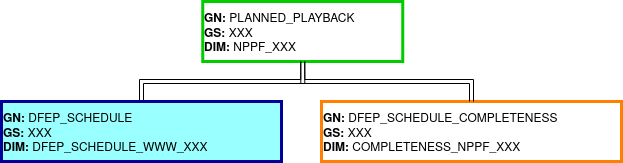
\includegraphics[width=150mm]{../fig/structure_ingestion_dfep_schedule.png}
	\caption{Structure of events inserted by the ingestion module for the MPL\_FS file}
	\label{fg:structure_ingestion_dfep_schedule}
  \end{center}
\end{figure}

The table \ref{tb:description_events_ingestion_dfep_schedule} shows the description of the events inserted by the ingestion.

\begin{landscape}
\begin{longtable}{|M{0.15\linewidth}|M{0.05\linewidth}|M{0.10\linewidth}|M{0.10\linewidth}|M{0.15\linewidth}|M{0.15\linewidth}|M{0.15\linewidth}|}
\hline \textbf{Gauge name} & \textbf{Gauge system} & \textbf{DIM signature} & \textbf{Insertion mode} & \textbf{Description} & \textbf{Start} & \textbf{Stop} \\ \hline
\textbf{DFEP\_SCHEDULE} & XXX & DFEP\_SCHEDULE\_SSS\_XXX & INSERT\_and\_ERASE\_per\_EVENT\_with\_PRIORITY (insert) & Event for representing the \textbf{DFEP schedule} & UTC value inside the start node & UTC value inside the stop node \\ \hline
\textbf{DFEP\_SCHEDULE\_COMPLETENESS} & XXX & \- COMPLETENESS\_NPPF\_XXX & INSERT\_and\_ERASE & Event for representing the \textbf{expectation of the DFEP schedule} & UTC value inside the start node & UTC value inside the stop node \\ \hline
\caption{Table describing the events associated to the ingestion}
\label{tb:description_events_ingestion_dfep_schedule}
\end{longtable}
\end{landscape}

\subsection{Ingestion details}

This section describes some ingestion details for inserting the data. In particular:

\begin{itemize} 

\item The correction of the generation time to avoid overriding data used for completeness analysis
  
\end{itemize}

\subsubsection{Correction of the generation time}

The generation time of the data extracted is one day before the validity start. This could be a problem as the processor of the ORBPRE files could override this data.

To solve this issue the processor changes the generation time to be the validity start.
